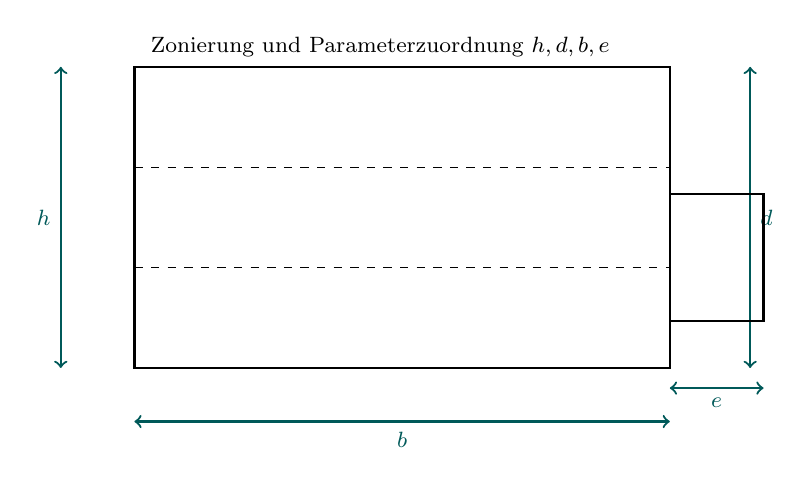
\begin{tikzpicture}[scale=0.85, every node/.style={font=\footnotesize}]
\draw[thick] (0,0) rectangle (8,4.5);
\draw[dashed] (0,1.5)--(8,1.5);
\draw[dashed] (0,3.0)--(8,3.0);
\draw[<->,teal!70!black,thick] (-1.1,0)--(-1.1,4.5) node[midway,left]{$h$};
\draw[<->,teal!70!black,thick] (0,-0.8)--(8,-0.8) node[midway,below]{$b$};
\draw[<->,teal!70!black,thick] (9.2,0)--(9.2,4.5) node[midway,right]{$d$};
\draw[thick] (8,0.7) rectangle (9.4,2.6);
\draw[<->,teal!70!black,thick] (8,-0.3)--(9.4,-0.3) node[midway,below]{$e$};
\node[anchor=west] at (0.1,4.8) {Zonierung und Parameterzuordnung $h,d,b,e$};
\end{tikzpicture}
